\javalstset{}{}
\section{Einleitung}
\label{sec:einleitung}
Als Abschlussübung der Vorlesung \emph{Aktuelle Themen der Dienstleistungsinformatik} im Wintersemester
 2012/13 an der TU-Dortmund sollten die teilnehmenden Studenten ein Projekt zum Thema Webservices
 durchführen. Dieser Bericht erläutert nun im Detail, wie das Projekt \textit{Kontakte} durchgeführt wurde.

In Kapitel \ref{sec:einleitung} wird zunächst die genaue Aufgabenstellung erläutert, welche das
 eigentliche Projektziel darstellt. In diesem Zusammenhang werden auch erste Überlegungen zur Projektplanung
 und -struktur aufgeführt.

Daraufhin werden in Kapitel \ref{sec:projektbausteine} die konkreten Projektbausteine behandelt. Zunächst
 werden die beiden Schnittstellen zu SAP und Google, welche auf Webservices basieren, im Detail erläutert,
 bevor es im Anschluss mit dem Thema der SIB-Programmierung weitergeht. Es wird erläutert, wie die
 SIB-Programmierung im Detail funktioniert und inwiefern die oben beschriebenen Schnittstellen in diesem
 Bereich ihre Anwendung finden.

Kapitel \ref{sec:jabc} beschäftigt sich mit dem konkreten Projektergebnis: dem fertigen jABC-Modell.
 Es wird der durch das Modell beschriebene Prozess im Detail erläutert und einige Fragen des Modelldesigns behandelt.

Abschliessend folgt in Kapitel \ref{sec:beurteilung} die konkrete Betrachtung der Projektergebnisse,
 um den Erfolg des Projektes zu beurteilen. 


\subsection{Projektbeschreibung}
Als Grundlage für die Aufgabenstellung diente ein fiktives Szenario in Form einer Umstellung der
 informationstechnischen Infrastruktur eines Unternehmens. Konkretes Thema für dieses Projekt war die
 Migration von kontaktbezogenen Stammdaten aus der Datenbank von SAP in das System von Google.
Für die Migration mussten drei Gruppen von Kontakten behandelt werden:
\begin{itemize}
	\item Kunden
	\item Liferanten
	\item Angestellte.
\end{itemize}
Die Migration selbst sollte dabei nicht der trivialen Strategie folgen, alle vorhandenen Kontakte
 in einem Prozess komplett zu kopieren.
Aufgrund der Existenz von sogenannten \gaensefuesse{Karteileichen} in der Datenbank von SAP, wurde
 eine Strategie vorgegeben, welche eine Migration nur bei Bedarf vorsieht.
Dadurch wird garantiert, dass das System von Google nur Kontaktdaten enthält, welche aktiv von dem
 Unternehmen genutzt werden.\\
Die Migrationsstrategie behandelt demnach nur einen einzelnen Kontakt und gliedert sich in drei Teile.
Zunächst muss im System von Google überprüft werden, ob der gewünschte Kontakt schon migriert worden ist.
Ist dies der Fall, so ist findet keine erneute Migration statt und der Prozess ist beendet.

Falls der gesuchte Kontakt nicht im System von Google existiert, wird versucht, diesen in der Datenbank
 von SAP zu finden und im Anschluss nach Google zu übertragen.
Da es bei einer Suche nach einem Kontakt, abhängig von den Kriterien, sowohl bei Google als auch bei SAP
 dazu kommen kann, dass mehrere Ergenisse zurückgeliefert werden, muss es dem Nutzer möglich sein, den
 gewünschten Kontakt aus dieser Ergebnisliste manuell auszuwählen.
In diesem Fall endet der Prozess mit einer erfolgreichen Migration von SAP nach Google.

Zudem muss die Tatsache abgedeckt sein, dass der gesuchte Kontakt ein gänzlich neuer ist, welcher bisher
 noch in keiner Datenbank auftaucht. Dann soll der Kontakt nach manueller Dateneingabe bei Google angelegt werden.

\subsection{Erste Überlegungen}
Damit eine effiziente Projektplanung gewährleistet werden kann, muss zunächst die Aufgabenstellung
 analysiert werden.
Das Ziel dieser Analyse ist es zunächst, Bereiche zu identifizieren, welche unabhängig bearbeitet werden können.
Dies unterstützt die Aufgabenverteilung an die einzelnen Projektmitglieder und legt deren Verantwortungsbereiche fest.

Da diese Teilbereiche im Projektzusammenhang jedoch an einigen Stellen miteinander interagieren sollen, müssen
 zudem geeignete Schnittstellen an den Berührungspunkten definiert werden.
 
Zudem gilt es auch, sich am Anfang der Planung über einzusetzende Technologien zu einigen, welche die Entwicklung unterstützen.

\subsubsection{Projektstruktur}
Aufgrund der Aufgabenstellung lassen sich die beiden Schnittstellen zu den Datanbanksystemen leicht als zwei
 unabhängige Bereiche identifizieren.
Ein weiterer Bereich ergibt sich durch die Tatsache, dass Nutzereingaben behandelt werden müssen.
Die Erstellung von GUI-Elementen bildet also den dritten Bereich des Projektes.

Diese soeben definierten Unterstrukturen der Software finden ihre Verwendung in der SIB-Programmierung, dessen
 Ergebnis das Produkt des Projektes darstellt: das jABC-Modell.
Somit wird der letzte eigenständige Bereich durch die Generierung dieser SIBs klassifiziert.
Die Abbildung \ref{fig:projektaufbau} zeigt eine sich daraus ergebene Projektstruktur.

\begin{figure}[h!t]
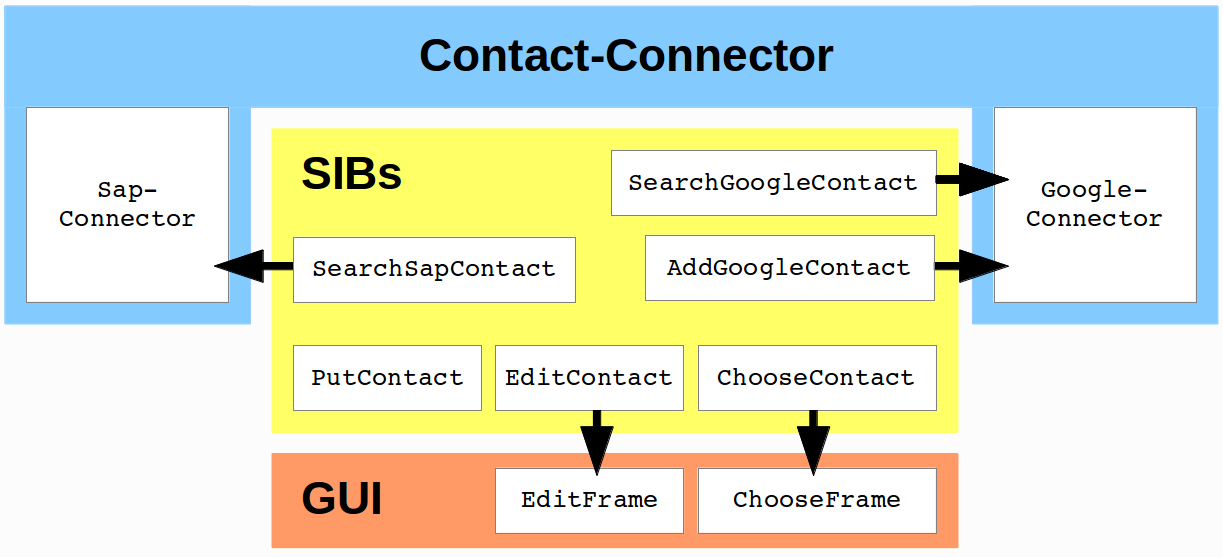
\includegraphics[width=\textwidth]{Bilder/projekt_aufbau.png}
\caption{Projektaufbau}
\label{fig:projektaufbau}
\end{figure}
	
\subsubsection{Das \lstinline{Contakt}-Objekt als Schnittstelle}
Die Verwendung der Unterstrukturen in der SIB-Programmierung macht es notwendig, eine geeignete
 Kommunikationsschnittstelle zu definieren.
Die Aufgabenstellung macht deutlich, dass der primäre Gegenstand des Prozesses ein \lstinline{Contakt}-Objekt ist.
Kontaktdaten werden eingegeben und an die Programmteile weitergegeben, welche die Kommunikation mit den
 externen Datenbanken realisieren.
Daraufhin wird eine Liste von \lstinline{Contakt}-Objekten zurückgeliefert und ein ausgewählter Kontakt wird
 dann bei Google gespeichert.
 
Ein einziges \lstinline{Contakt}-Objekt kann also als Schnittstelle genutzt werden, wenn es hinreichend klar definiert ist.
Das heißt, dass eine Abbildung gefunden werden kann, welche die Attribute des \lstinline{Contakt}-Objektes mit den speziellen
 Strukturen der externen Datenbanken verknüpft.
Aus diesem Grund wurden für das Projekt Attribute gewählt, welche in beiden Datenbanken verwendet werden.
Insbesondere musste auch darauf geachtet werden, dass diese Attribute in allen drei Gruppen (Kunde, Lieferant,
 Angestellter) vorhanden sind.
Aus diesem Überlegungen wurde das \lstinline{Contakt}-Objekt mit folgenden Attributen definiert:
\begin{itemize}
	\item Vorname, Nachname, Firma
	\item Adresse (Strasse, PLZ, Ort)
	\item Telefonnummer, Emailadresse
\end{itemize}
Desweiteren enthält das Kontaktobjekt die eindeutigen Identifikationkennungen des SAP- und Google-Systems.
Zum einen kann dadurch die Herkunft eines Kontaktes verfolgt werden und zum anderen bietet es Möglichkeiten
 zur Implementierung einer komplexeren Migrationsstrategie.
Es kann dann zum Beispiel automatisch geprüft werden, ob ein Kontakt bereits migriert wurde oder ob dieser
 Kontakt überhaupt aus dem SAP-System stammt.
	
\subsubsection{Eingesetzte Technologien}
Es wurden einige Entscheidungen über zu verwendende Tools getroffen, um die Projektarbeit und die
 Implementierung zu unterstützen.
 
Zum einen wurde das Versionskontrollsystem \emph{Git} verwendet.
Neben einer zentralen Speicherung aller Projektdaten unterstützt \emph{Git} die kooperative Implementierung des Programmcodes.
Änderungen an verschiedenen Teilen der Software werden automatisch zu einer neuen Version zusammengefasst.

Um die einzelnen Programmbausteine ausreichend zu testen, um deren Funktion zu verifizieren, wurde zudem das
 Test-Framework \emph{JUnit} verwendet. Dadurch ist es beispielsweise möglich, die Suchfunktion der Konnektoren ausgiebig
 zu testen, bevor diese in der SIB-Programmierung ihre Verwendung finden.

Ein weiteres Tool, welches zur Unterstützung für den Softwarelebenszyklus verwendet wurde, ist \emph{Apache Maven}.
Es bietet den Vorteil, dass im Anschluss an die Kompilation automatisch \emph{JUnit}-Tests ausgeführt werden, bevor
 die Software zu einem grossen Paket geschnürt wird.
 \emph{Apache Maven} trägt ausserdem dafür Sorge, dass alle Abhängigkeiten, welche für die Ausführung der Software
  notwendig sind, mit in das erzeugt Programmpaket gepackt werden.
 Dies erleichtert die anschliessende Verwendung im jABC, da nur ein einziges Paket eingebunden werden muss.

Dazu muss jedoch gesagt werden, dass das Zusammenschnüren von einem großen Paket im allgemeinen nicht empfohlen wird.
Falls eine einzelne Komponente des Pakets aktualisiert werden soll, muss das ganze Paket neu erstellt werden. 

\section{Unsere Projektbausteine}
\label{sec:projektbausteine}
Dieses Kapitel beschreibt die Projetbausteine und weist auf die entdeckten Probleme und getroffnen Entscheidungen hin.
